% !TEX root = master_thesis.tex

%==============================================================================
\chapter{Introduction}
\label{sec:intro}
%==============================================================================
\section{The Standard Model of Particle Physics}
A summary of the SM can be found in figure \ref{fig:sm}. 

\begin{figure}[htbp]
	\centering
	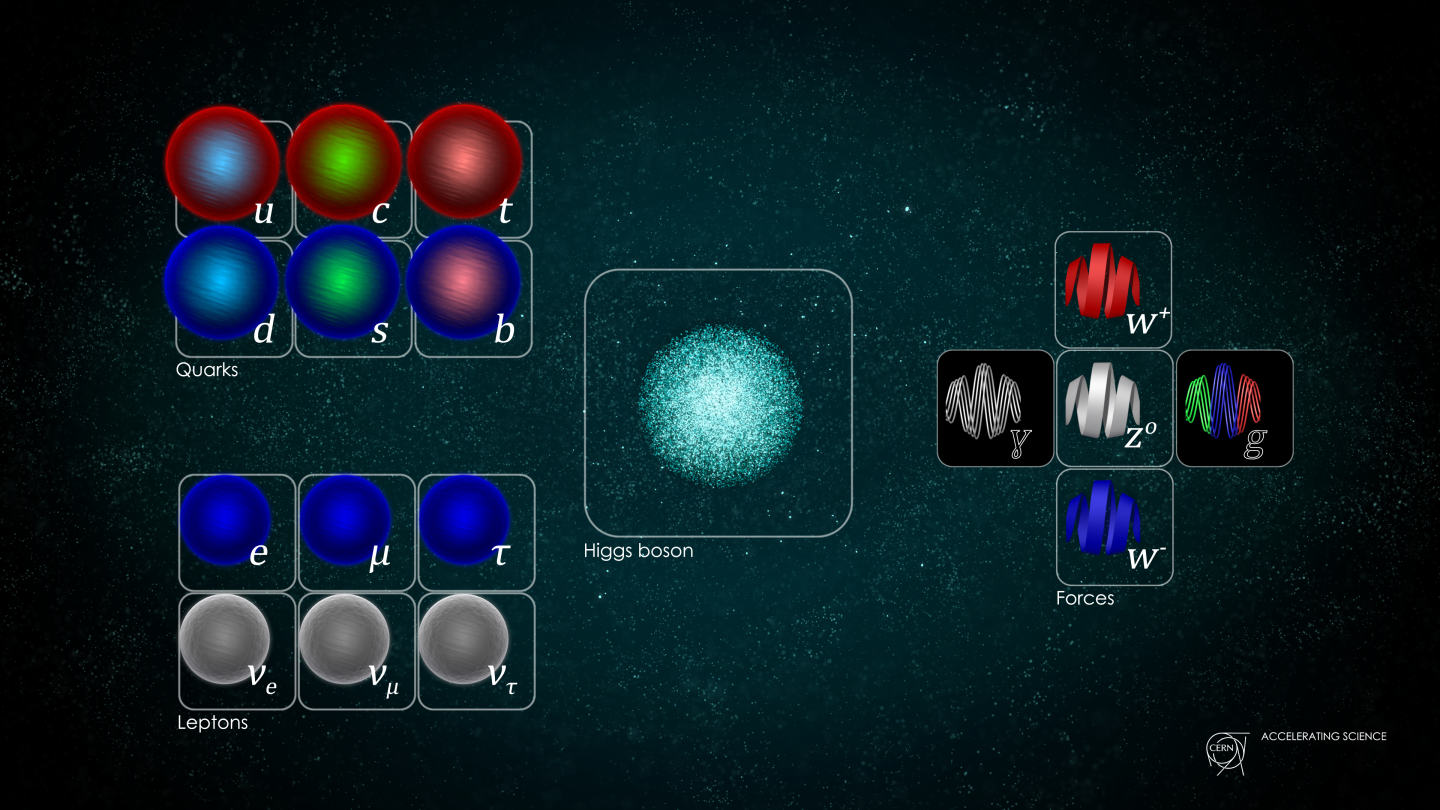
\includegraphics[width=\linewidth]{sm}
	\caption{Standard Model of Particle Physics, taken from \cite{sm}}
	\label{fig:sm}
\end{figure}
\section{Photoproduction of Pseudoscalar Mesons}
$$\int_0^\infty\frac{\sin \alpha\beta x}{\gamma x}$$
\section{Polarization Obervables and the Complete Experiment}
bla
\section{Motivation and Structure of this Thesis}
bla